
\documentclass[11pt]{article}
\usepackage{UF_FRED_paper_style}

%% ===============================================
%% Setting the line spacing (3 options: only pick one)
% \doublespacing
% \singlespacing
\onehalfspacing
%% ===============================================

\setlength{\droptitle}{-5em} %% Don't touch

% TITLE:
\title{RBE 594: EnterTrainer Capstone Project
% \thanks{Selected Paper prepared for presentation at the 201X Agricultural \& Applied Economics Association Annual Meeting}
}

% AUTHORS:
\author{Troy Denning\\% Name author
    \href{mailto:tjdenning@wpi.edu}{\texttt{tjdenning@wpi.edu}} %% Email author 1 
\and Christopher Grontkowski\\% Name author
    \href{mailto:cfgrontkowski@wpi.edu}{\texttt{cfgrontkowski@wpi.edu}} %% Email author 1 
\and Lanhao Mao\\% Name author
    \href{mailto:firstauthor@wpi.edu}{\texttt{lmao@wpi.edu}} %% Email author 1 
\and Daniel Roberts\\% Name author
    \href{mailto:firstauthor@wpi.edu}{\texttt{daroberts@wpi.edu}} %% Email author 1 
\and Peter Subacz\\% Name author
    \href{mailto:pasubacz@wpi.edu}{\texttt{pasubacz@wpi.edu}} %% Email author 1 
    }
    
% DATE: (due date of the paper)
\date{April 27, 2020}

\begin{document}
{\setstretch{.8}
\maketitle
% %%%%%%%%%%%%%%%%%%
\begin{abstract}
% CONTENT OF ABS HERE--------------------------------------
Domestic canines have an unfortunate disadvantage when their owners have work or other activities that limit their pet engagement availability for extended periods. Many canines owners have a desire to increase the opportunities their pets have for lively, engaging, quality entertainment and exercise. The EnterTrainer allows time-restricted pet owners to have their pets physically engaged through a continuous game of fetch when the owner is unable to attend to the canine. The system autonomously works to maximize safety and ease of use. The SLAM and path planning module and quality mobility solution are designed to autonomously navigate the interior of a house with minimal disturbances to its environment. Balls are launched via the use of a trajectory launcher capable of generating multi trajectories and determining if a trajectory will adversely affect the environment, potentially damaging fragile objects in the house. With only a few essential sensors, a sturdy but quick frame, and a custom-built software package, this system can keep the beloved canine pets physically engaged with no intervention required by their owners.

% END CONTENT ABS------------------------------------------
\noindent
\textit{\textbf{Keywords: }%
RRT*; SLAM; Gazebo; ROS; Path Planning; Spring; Electromagnet; Point Cloud Library; Newtonian Physics; Non-holonomic; Ackerman Steering; Trajectory Planning.} \\ %% <-- Keywords HERE!

\end{abstract}
}

\section{Introduction}
% --------------------

The five authors of this report are all students attending WPI's Robotic Masters Program. This report presents the work and research conducted during the Capstone course project. The Capstone course required that the team select a project of their choice and follow a condensed/accelerated systems engineering design process. The limited time constraints of the class reduced the ability to follow a full plan, build, simulate and test process. The delivery for the course was thus a list of agreed upon tasks that could reasonably be completed during the time constraints of the course.

This paper is organised into the following sections: Objective \& Design Concepts, Requirements, Hardware, Software System Architecture, and Simulation.

\section{Objective, Design Concepts, \& Requirements}
% --------------------
The objective of this project is to create a system that can autonomously entertain and exercise canine pets when caretakers are unable to attend to the needs of the canine. 
%%%%%%%%%%%%%
The objective of the solution is to physically be able to swiftly move about a single floor in a home or apartment and launch a tennis ball in a safe manner inside the environment.
%%%%%%%%%%%%%
The requirements for the EnterTrainer were derived from the perspective of the aforementioned busy, indoor domestic canine owners. As the pet owner is busy, it was assumed the system would operate with little to no human input. It was also assumed that the home owner would not appreciate insuring home damage from tennis balls being thrown around nice flower vases, ornate lamps, or expensive electronics.   


\subsection{Concepts of Operations}
% --------------------
The goals and objectives of the system are:
The robot is a mobile entertainer for household canine pets. The objective of this system is to provide a method of entertainment via autonomous tennis ball launching.
\begin{itemize}
	\item The system will be able to launch tennis balls within an indoor environment for a dog to find and retrieve. 
	\item The system will be capable of finding tennis balls and internally reloading them for future use.
	\item The system will be able to learn from its surroundings to create a map of the environment to calculate safe trajectories.
	\item The system will light light, durable, and acceptable for children.
	\item The system will be visually appealing.
	\item The system will be designed to minimize damage to itself and its operating environment. 
	\item No small parts, and not capable of splintering during average rough housing.  This will allow increased safety for small children.
	\item No easily accessible sharp edges.
	\item Sounds from the robot need to be less than or equal to continuous 65-decibel. This is to reduce hearing loss after prolonged proximity to the system. 
\end{itemize}  
\subsection{Design Concepts}
% --------------------
Several design concepts were evaluated for each subsystem within the Entertrainer. Each design concept was evaluated and assigned a value to help choose the best concept. 
\subsubsection{Design Concept - Locomotion}
The locomotion design concepts that we evaluated were mechanum wheels, Tracks, Quadruped, BB8, Ackerman, and Roomba style. We decided to choose the Roomba style robot based on its simplicity, stability, power consumption, and cost. The two drive wheels coupled with a back caster wheel for stability provides a proven locomotion solution for indoor environments. 
\subsubsection{Design Concept - Cannon}
The cannon design concepts that we evaluated were the throwing arm, air pressure cannon, spring loaded cannon, little league pitching machine, and the double spinning wheel launcher. We decided on the spring loaded cannon mainly based on the safety, simplicity, and adaptability. 

\subsection{System Level Requirements}
% --------------------
Mapping and Localization Requirements
\begin{itemize}
    \item The system  shall be able to autonomously explore and create a map of an indoor environment.
    \item The system  shall be able to update the map to reflect obstacle changes within the environment.
    \item The system  shall be able to resolve its location within a mapped environment.
\end{itemize}
Path planning requirements
\begin{itemize}
    \item The system shall be able to navigate autonomously around a single level plane environment.
    \item The system shall be able to plan a path to given waypoints.
\end{itemize}
Motion Control Requirements
\begin{itemize}
    \item The system shall be able to follow the path generated with internal motion controllers.
\end{itemize}
Object Recognition
\begin{itemize}
    \item The system shall be able to detect and classify objects with a 10 meters of the device location (People, Dogs, Couches, Lamp, TV, Cabinet, Tree, Window, Vase, etc).
\end{itemize}
Projectile Trajectory Planning
\begin{itemize}
    \item The system shall be able to predict projectile trajectories.
    \item The ball launcher shall only launch balls in a safe manner.
\end{itemize}
Physical
\begin{itemize}
    \item The system shall be water resistant.
    \item The system shall be stable when interacting with canines
\end{itemize}
Locomotion
\begin{itemize}
    \item The system shall be able to traverse across hardwood, carpet, tile, rugs, concrete, or dirt without getting stuck or snagged
    \item The system shall be capable of backing up and maneuvering around static and dynamic obstacles
\end{itemize}
Launcher
\begin{itemize}
    \item The system shall be able to launch a ball a maximum horizontal distance of 15 Feet.
    \item The system shall be canine reloadable.
\end{itemize}

\section{Hardware}
% --------------------
This section covers the hardware associated with the EnterTrainer system. It consists of a locomotion chassis and a cannon to launch tennis balls. The locomotion chassis is a two wheel drive system with a caster wheel in the back for stability. This setup gives the necessary degrees of freedom to navigate around the house, avoid obstacles, and still provide the necessary stability for firing a tennis ball. 
\subsection{Locomotion}
The EnterTrainer Locomotion system was modeled mimicking the locomotion of the iRobot's Roomba. This system was selected not only for it's long lasting track record of home navigation, but also because it fared better when compared to other locomotion platforms.
The requirements that were assigned to the locomotion system, included stability, sound levels, and maneuverability.
The solution for the locomotion platform is presented in Figure \ref{Locomotion}.

%-- Add a photo of the "tennis ball"
\begin{figure}[H]
    \centering
        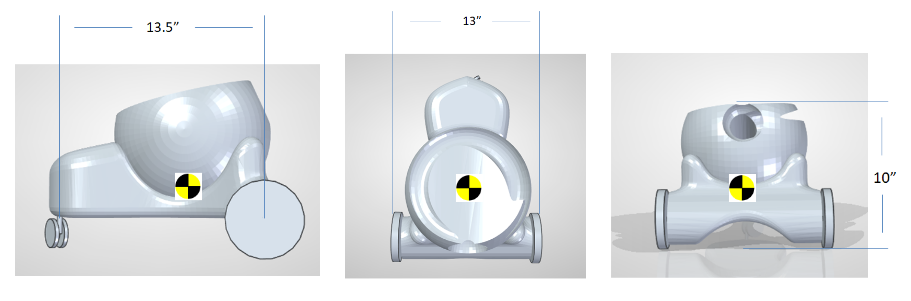
\includegraphics[scale=0.6, angle =0]{figures/Center of mass.PNG}
    \caption{Locomotion Platform.}
    \label{Locomotion}
\end{figure}

It implements the three wheeled locomotion system of the Roomba in a wide and stable layout. This provides the ability for the canine to reload the launcher without the potential of knocking it over. The structure includes room for all the tennis balls, sensors, motors, and computing hardware that is needed. 

\subsection{Tennis Ball Launcher}
% --------------------
The EnterTrainer has a requirement to launch a tennis ball at a distance of 4.5 meters. To accomplish this requirement, a ball launcher needed to be designed. Many options were considered for launching the ball including an air presser cannon, a robotic arm, and a kinetic wheel launcher similar to a pitching machine, but a spring loaded cannon scored the highest when impacts of sound, scores of power, weight, and visual appeal were considered.

A spring loaded cannon design required the combination of a proper sized spring and launching mechanics. The ball selected was a dog toy squeaker tennis ball just under 50.8 mm diameter. The ball fit nicely inside a 50.8 mm drain pipe as the launcher tube. 


\subsubsection{Spring Sizing}
% --------------------
A spring analysis was performed to verify the launcher could meet system requirements.The approach the team took to solving for the spring dimensions was a mixture of the Newtonian trajectory equations and the potential and kinematic energy balance equations. The known parameters of the trajectory; namely: the angle of attack of 45 degrees, and the desired maximum trajectory distance were used to establish the maximum required exit velocity of the tennis ball. The equation used can be seen in Figure \ref{VE} \cite{5}

\begin{figure}[H]
    \centering
        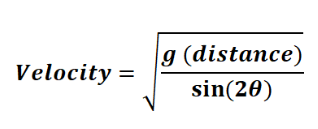
\includegraphics[scale=.8, angle =0]{figures/Velocity.PNG}
    \caption{Velocity Equation.}
    \label{VE}
\end{figure}

where "g" is the gravitational constant, "distance" is the  distance the ball will travel before hitting the ground (4.5 meters), and $\theta$ is the launch angle of the ball (45 degrees). The resulting required velocity for the spring to generate was 6.7 m/s.
This velocity was then converted to kinetic energy and compared to the spring potential energy equations, both seen in Figure \ref{EE} \cite{5}


\begin{figure}[H]
    \centering
        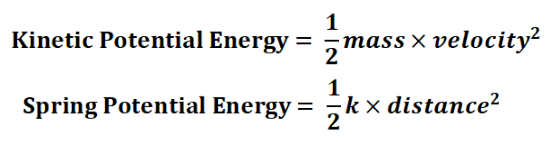
\includegraphics[scale=.8, angle =0]{figures/Energy.PNG}
    \caption{Energy Equations.}
    \label{EE}
\end{figure}
Where "velocity" is the same velocity calculated for the trajectory, "mass" is the mass of the ball, "k" is the spring constant, and "distance", in this case, is the distance the spring needs to be compressed. Equating the two energy models provided one equation with two unknowns. The team needed to specify either the spring constant, or the distance the spring would need to travel. The team selected the spring distance as the parameter to fix. The distance selected was 76 mm. This distance seemed good for allowing whatever pulled the spring back a little variance to reach the needed spring compression.

The team also wanted the ability to meet the 4.5 m requirement for higher trajectory paths. The higher paths could be utilized if the ball needed to travel over a couch or large piece of furniture. Thus the length for the spring was extended to about double the 76 mm selection. However the distance used for determining the K factor for the spring would still be the original 76 mm. The results provided a K factor of 46 g/mm.

The spring K factor was used to define the physical characteristics of the spring using the equation presented in figure \ref{EE}. \cite{4}

\begin{figure}[H]
    \centering
        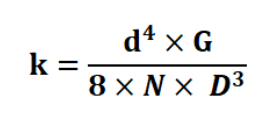
\includegraphics[scale=.8, angle =0]{figures/K.PNG}
    \caption{Spring K Factor Equation.}
    \label{k}
\end{figure}
Where "d" is the wire diameter, "D" is the mean Spring Diameter, N is the number of active coils in the spring and G is the Modulus of Rigidity of the spring material. There were a number of the spring constant parameters that could not be altered including the OD of the spring and the spring marital. The spring material needed to be resistant to dog slobber, and the OD of the spring needed to fit nicely in the launch tubule. With limited options of off the shelf springs, the team selected an available spring with the following characteristics.
\begin{itemize}
    \item Material- stainless steel
    \item Wire diameter -.3 mm 
    \item Spring length - 210 mm
    \item Number of active coils - 8
    \item Spring OD - 47.6 mm
\end{itemize}
This spring had a calculated spring constant k of 83.8 g/mm. This was more then what was needed but could work for a proof of concept. 

\subsubsection{launcher Development}
The cannon assembly consists of a linear actuator, spring, electromagnet, cannon nozzle, and an adapter to hold everything together; as seen in Figure \ref{LA}.


\begin{figure}[H]
    \centering
        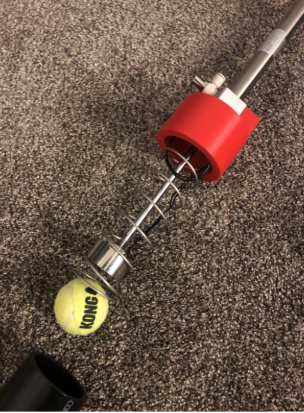
\includegraphics[scale=.80, angle =0]{figures/Launcher.PNG}
    \caption{Cannon Assembly Components.}
    \label{LA}
\end{figure}

The electromagnet needed to be strong enough to hold back .453 kg based on the original spring constant and anticipated spring length. This calculation would ensure the magnet will be able to hold the spring when it was fully compressed.   


The firing mechanism uses the electromagnet at the end of a linear actuator to extend and attach to a plate at the end of the spring. Once the electromagnet is attached to the plate at the end of the spring, the linear actuator can be retracted to a desired specific length. To launch the ball, the electromagnet is deactivated and thus releasing the spring.



The prototype was constructed and attached to an end-effector of a Fanuc 200iD/7l robot. The cannon tube vector direction could be controlled by the robotic plc system along with both the liner actuator and electromagnet. The prototype system was tested to verify the ball would launch 4.5 mm. The results of the testing are presented in Figure \ref{Cannon Angle cannon test data}.

\begin{figure}[H]
    \centering
        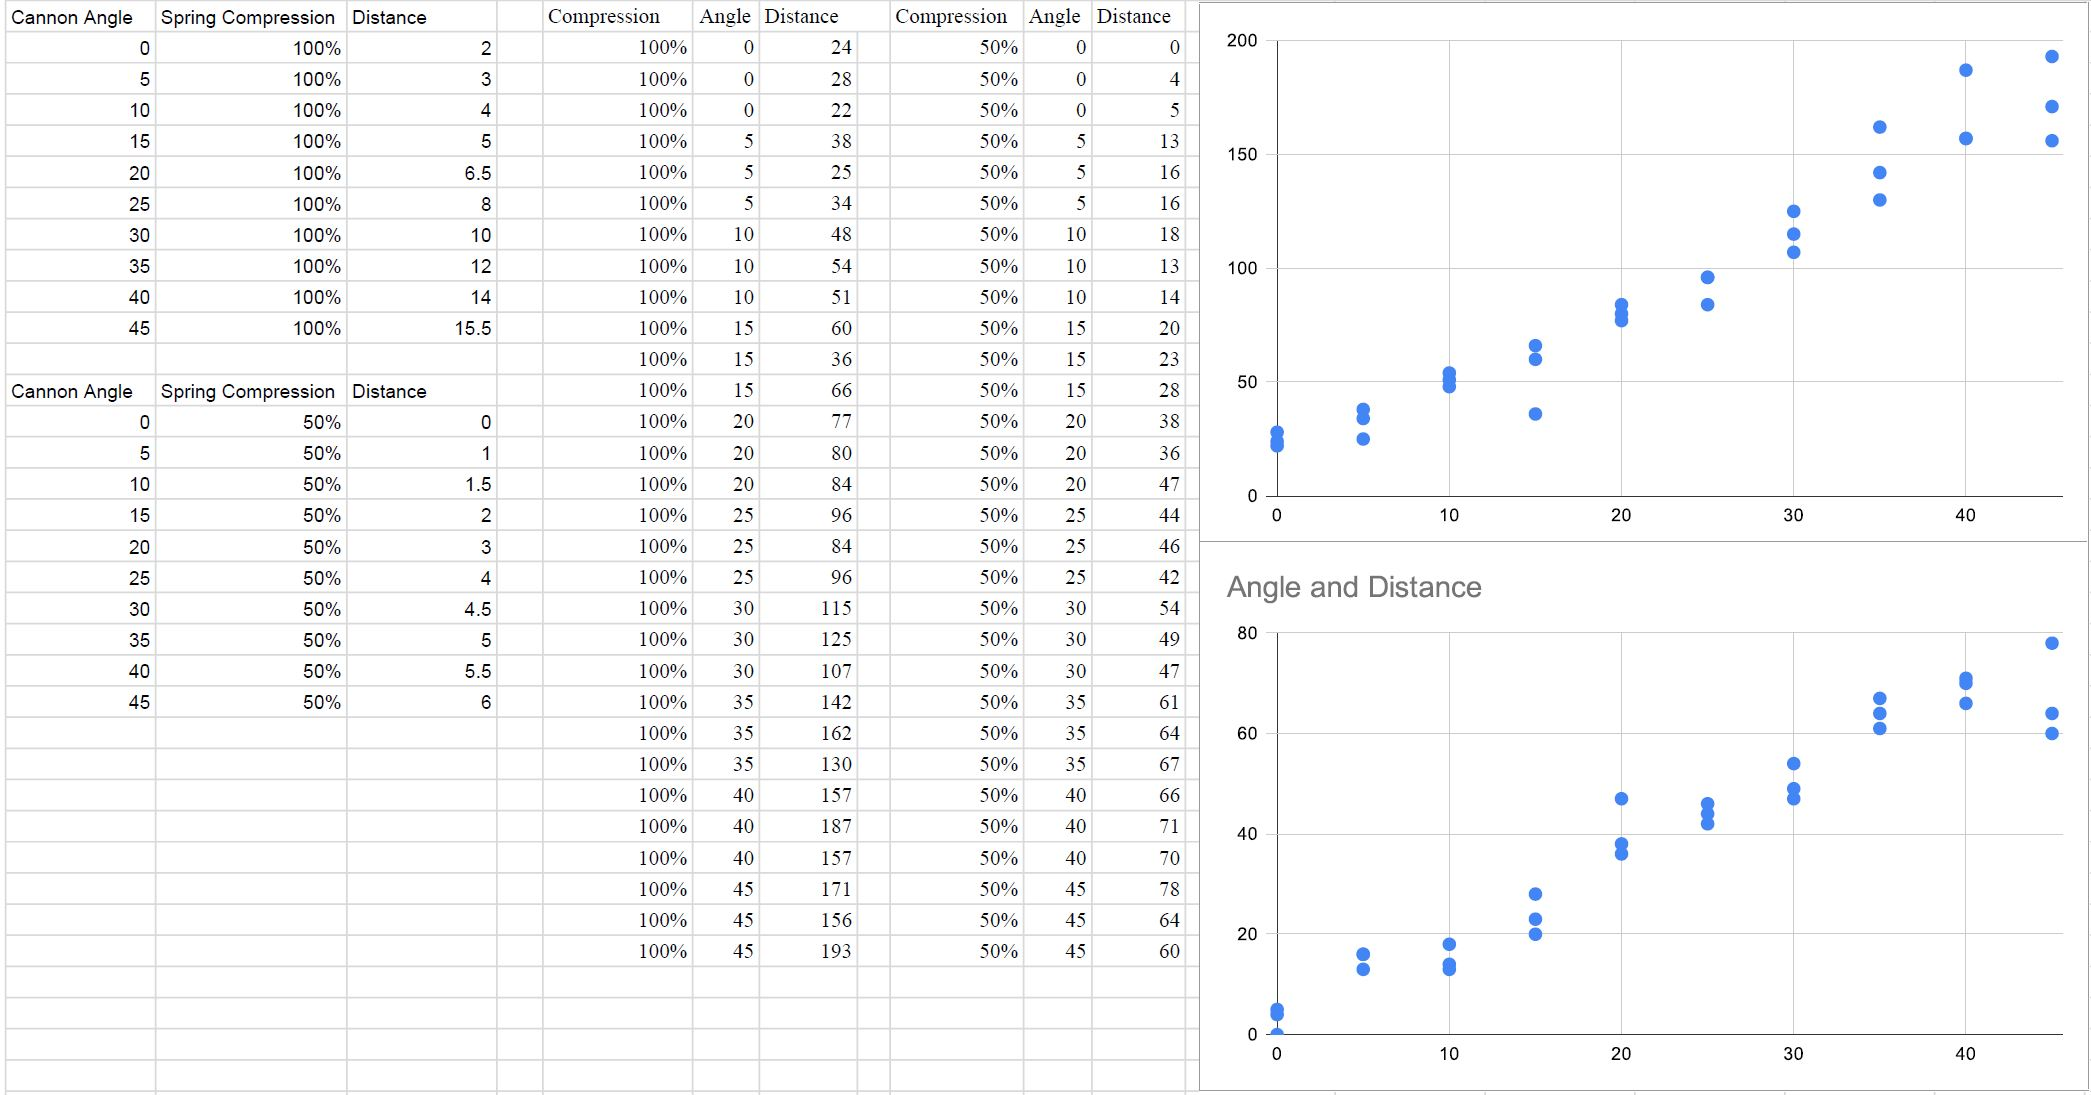
\includegraphics[scale=.42, angle =0]{figures/cannon_prototype_angle_fireing_distance.JPG}
    \caption{Cannon angle test data.}
    \label{Cannon Angle cannon test data}
\end{figure}

From the results of the test the team realised there was a significant loss of energy. Upon investigation it was seen that the weight of the steel plate attached to the end of the spring did not make it into the spring potential energy equation. This added weight and other factors soaked up a large portion of the anticipated spring energy and decreased the exit velocity by more then half. Another factor that soaked up the spring energy was the friction of the ball and spring scraping the sides of the launch tube. We also investigated the actual spring constant to see how the calculated spring constant compared to the actual spring. The results of the study can be seen in Figure \ref{me}.

\begin{figure}[H]
    \centering
        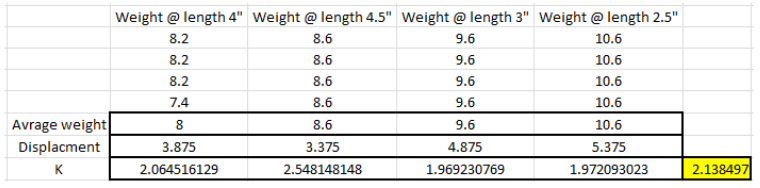
\includegraphics[scale=.8, angle =0]{figures/mes.PNG}
    \caption{Measured Spring K Factor.}
    \label{me}
\end{figure}

The large deviance in the calculated vs measured spring constant can potently be tied to the less accurate scale used in the test. It may also be due to the material constant value used in the calculation. Nevertheless, testing the spring proved that the spring potential energy was not as large as calculated.

The accuracy of the tennis ball cannon varied with the distance that the ball was fired. The cannon became less accurate the further the ball was shot. Some of this inaccuracy is due to the friction between the spring and the cannon tube as well as the other variable losses in the potential energy. 

Despite the apparent energy losses in the system, the launcher preformed very well. And because the system was able to successfully reach a maximum trajectory distance of 4.5 m, the team feels confident that the spring loaded canon is still the best option for launching the ball. The current prototype shows there are some improvements that can be made, but as a proof of concept it was a success. 

\section{Software System Architecture}
% --------------------
This section covers the software design, logic, and flow of the EnterTrainer system. There are four modules that run the EnterTrainer system: Mapping and Localization, Motion Planning, Trajectory Planning, and Launcher Controller. The system architecture design needed to be designed to satisfy the main functionalities of the robot, which are:
\begin{itemize}
	\item Explore the unknown indoor environment and build a cartesian occupancy map of the environment. 
	\item Use the map and various sensor readings to localize the robot within the indoor environment. 
	\item Update the map gradually if any obstacle changes overtime. 
	\item Plan a traversable path (satisfy the robot motion constraint) from robot's current location to given goal.
	\item Use motion controller to ensure the robot follows the path given.
	\item Generate trajectories that a ball will follow once launched.
	\item Collision check between trajectories and map point cloud data to identify if a trajectory is safe. 
	\item Calculate the impact energy imparted on a hit object. Update trajectories based on collision energy.
\end{itemize}
% --------------------
\subsection{Mapping and Localization}
The robot will be operated within two modes: the exploration mode and the operation mode. When the robot is introduced to a new environment, the robot will engage in the exploration mode where a full SLAM will guide the robot around the environment. After the indoor environment is fully mapped and identified, the robot can generate a Cartesian occupancy map to guide the robot in its normal functions. Within the operation mode, the robot will use the pre-build map to engage in self localization, map traversing and ball launcher trajectory planning. 

In the SLAM mode, the robot traverse around the environment until all corners of the indoor environment is mapped. In this project, the Gmapping SLAM package from the ROS navigation stack is used. Underlying the Gmapping package is a Rao-Blackwellized particle filter that takes in the odometry data from the robot mobile base as well as the 2D LiDAR scan to form a 2D binary occupancy grid of the environment. Although Gmapping provides a full solution of continuous grid mapping, the robot has to be given exploration goals so the robot can traverse every corner of the environment during mapping. To provide the robot with exploration goals, the team implemented a frontier finder to identify the most prominent "frontier", an unexplored free space edge of the current map, and direct the robot to explore using the motion planner described in the section below. In the preliminary testing, the frontier finder was implemented by grid searching the current occupancy map and identifying all connected open edges. However, the team has quickly realized that grid searching does not have nearly enough efficiency for multi-opening continuous frontier searching. Thus, the team implemented a second version by converting the occupancy map to black and white image matrix then search using OpenCV. The Canny edge detector is used to identify the edges between open space and unknown space. The longest edge is kept as the most open frontier to explore and then the centroid of that frontier edge is sent to the motion planner as the next exploration point. The figure below illustrates the frontiers identified in OpenCV and the exploration point sent to the robot.

\begin{figure}[H]
    \centering
        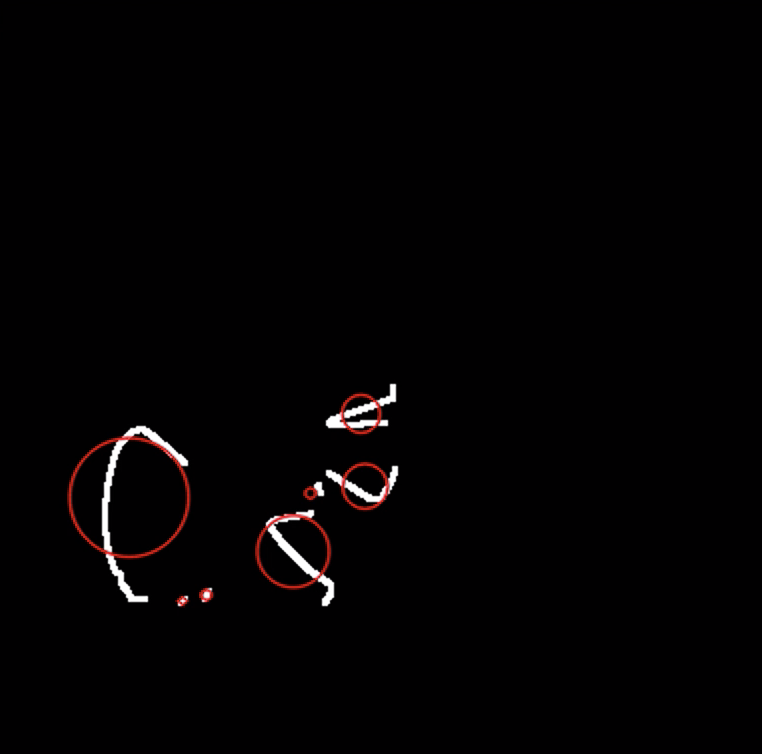
\includegraphics[scale=.4, angle =0]{figures/SLAM-1.png}
    \caption{Frontier identification in OpenCV.}
    \label{Frontier identification in OpenCV}
\end{figure}

\begin{figure}[H]
    \centering
        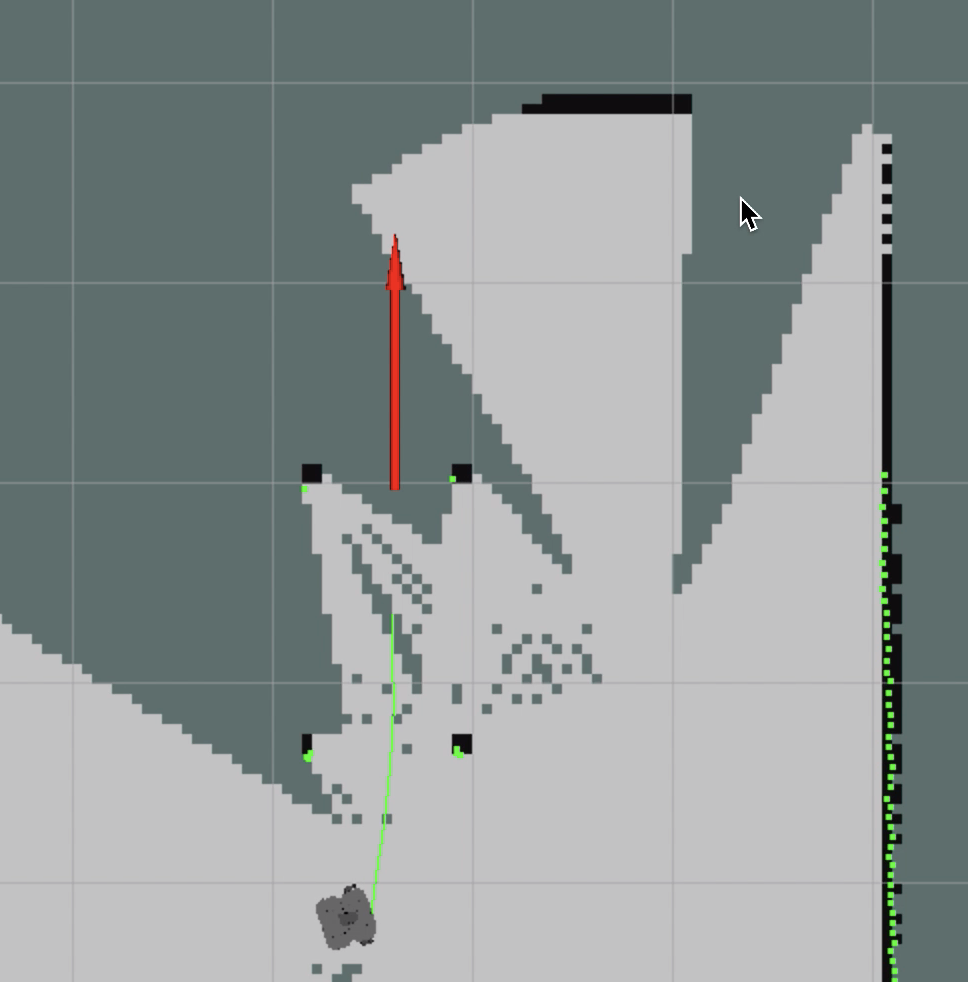
\includegraphics[scale=.4, angle =0]{figures/SLAM-2.png}
    \caption{Frontier frontier exploration goal update.}
    \label{Frontier frontier exploration goal update.}
\end{figure}


In the operation mode, the localization node will be continuously running while taking in sensor data from the LiDAR and encoder. The localization package receives the map of the environment from the map server and provide the transform between the the map global frame and the robot local frame. In this project, the team utilized the ROS Adaptive Monte Carlo Localization (AMCL) package as the localization filter. 

Although the localization can be operated smoothly given an accurate map of the environment, the indoor environment layout is sometimes volatile with high possibilities of both altered static obstacle and dynamic obstacle, which will make the original map an inaccurate source for environment traversal. Thus, an implementation of probabilistic map update is necessary to gradually update the occupancy map, reflecting the changed environment. Based on the Bayesian inference, the posterior probability consists of two sections: the prior probability and the likelihood probability for the current observable data. The Bayes theorem calculates the probability of current events given on prior beliefs. In a continuous event like localization and map update, based on the Markov assumption, the current observation is not based on the prior observation, thus, in the case of this project, the occupancy map has an update function of:

\begin{figure}[H]
    \centering
        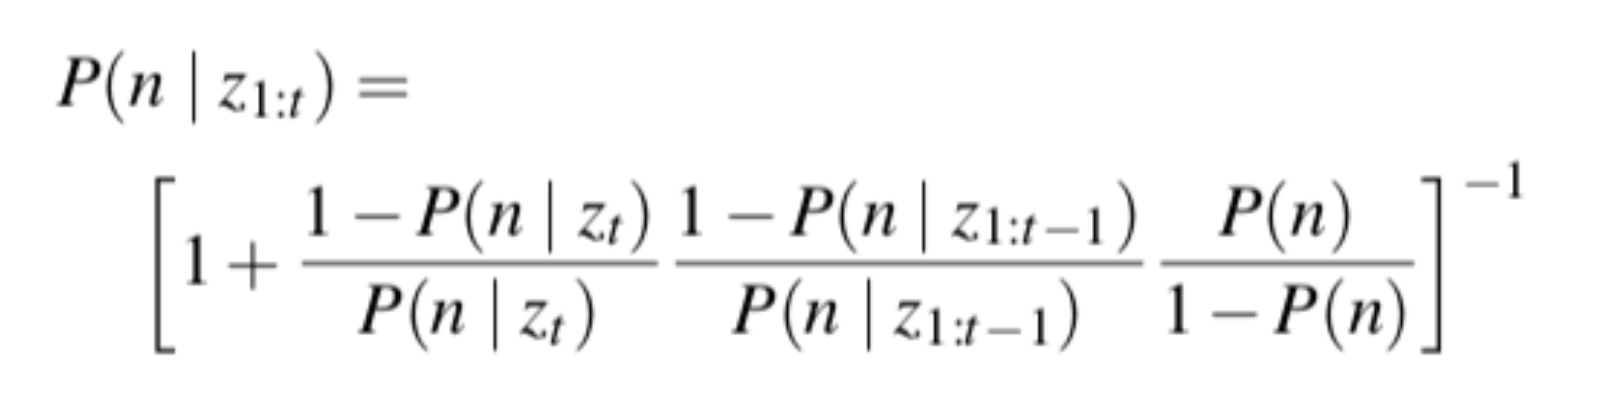
\includegraphics[scale=.3, angle =0]{figures/prob-1.png}
    \caption{Occupancy map update function.}
    \label{me}
\end{figure}

In this update function, it contains:
\begin{itemize}
	\item The prior probability P(n)
    \item The current measurement Zt 
    \item The previous estimation P(n $|$ z1:t-1)
\end{itemize}

Using the prior research in \cite{2} during the making of the Octomap, the update function can be evolved and represented by using log functions to speed up individual cell probability update since log update functions can be performed with addition instead of normal bayesian multiplication. Thus the update function can be rewritten as:

\begin{figure}[H]
    \centering
        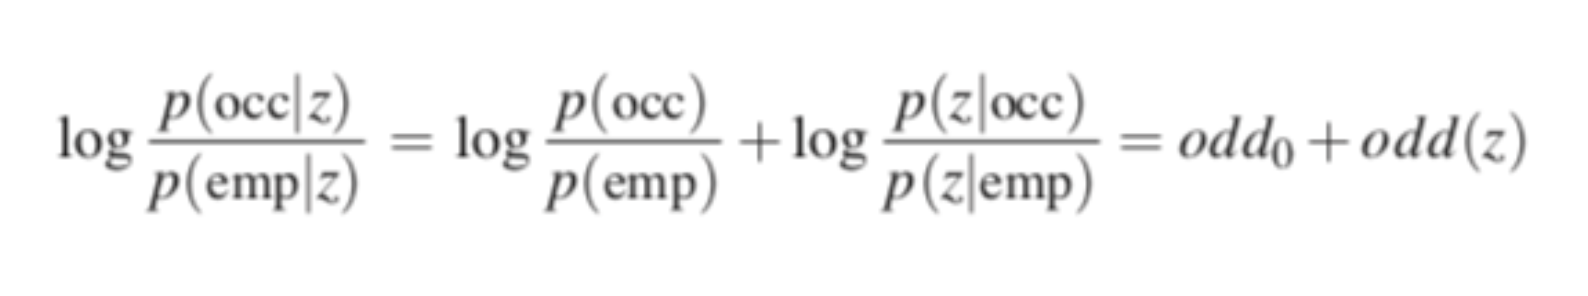
\includegraphics[scale=.4, angle =0]{figures/prob-2.png}
    \caption{Occupancy map log update function.}
    \label{me}
\end{figure}


The occupancy map model is initialized with an uniform probability of 0.5 for every cell. The occupancy of a cell is determined by the update function score where the cell is considered empty until the score is over a threshold (0.9 is used within the testing). Therefore, more number of occupied sightings than the empty sightings are required in order to alter the cell’s status. The problem occurs when in a long term map update, the empty cells will become more reluctant to sudden changes as the prior beliefs of emptiness has been reinforced a number of times. To combat this problem, \cite{3} proposed a solution of a clamping algorithm where an upper bound and a lower bound of prior belief is provided so the cell will not establish an unchangeable probability over time:

\begin{figure}[H]
    \centering
        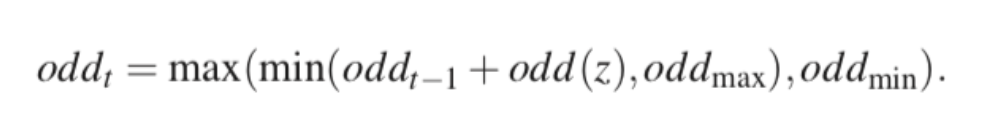
\includegraphics[scale=.5, angle =0]{figures/prob-3.png}
    \caption{Occupancy map update with bound limits.}
    \label{me}
\end{figure}

In this project's implementation, the maximum and minimum probabilities are kept between 0 and 1 so the map can quickly adapt to static obstacle changes within the environment if a small given number of consistent occupied observations are given. 
In order to update the map with current observation, a local occupancy map needed to be generated from the current laser scan. This can be accomplished by ray tracing every laser scan point to the sensor origin to identify the free space and the obstacle region. In this project, the team utilized the ROS Costmap 2D package in the navigation stack as it already provides the local occupancy map with a changeable obstacle padding radius. The probabilistic map update is called with a user defined frequency to ease the computation strain on the system. In the testing, the team used a frequency of 0.1 (update every 10 laser scan received).


\subsection{Motion Planning}
To plan a path between the current robot location and the given goal, RRT is chosen to be used as the path planning method in this project. Although RRT nor the RRT* can provide the optimality as well as grid searching methods such as A*, the shortest path guaranteed is not as important in this scenario. More, due to the nature of constantly changing goals for the robot, ie. following a dog that constantly changes directions, fast re-planning is necessary for the motion planner and only probabilistic path planning algorithms can provide such utility. Thus, the first implementation of the RRT path planning was developed and tested on a set of simulated indoor maps. The pseudo-code below explains the general algorithm of RRT from random point generation, to nearest neighbor search to new node and new edge adding. 

\begin{figure}[H]
    \centering
        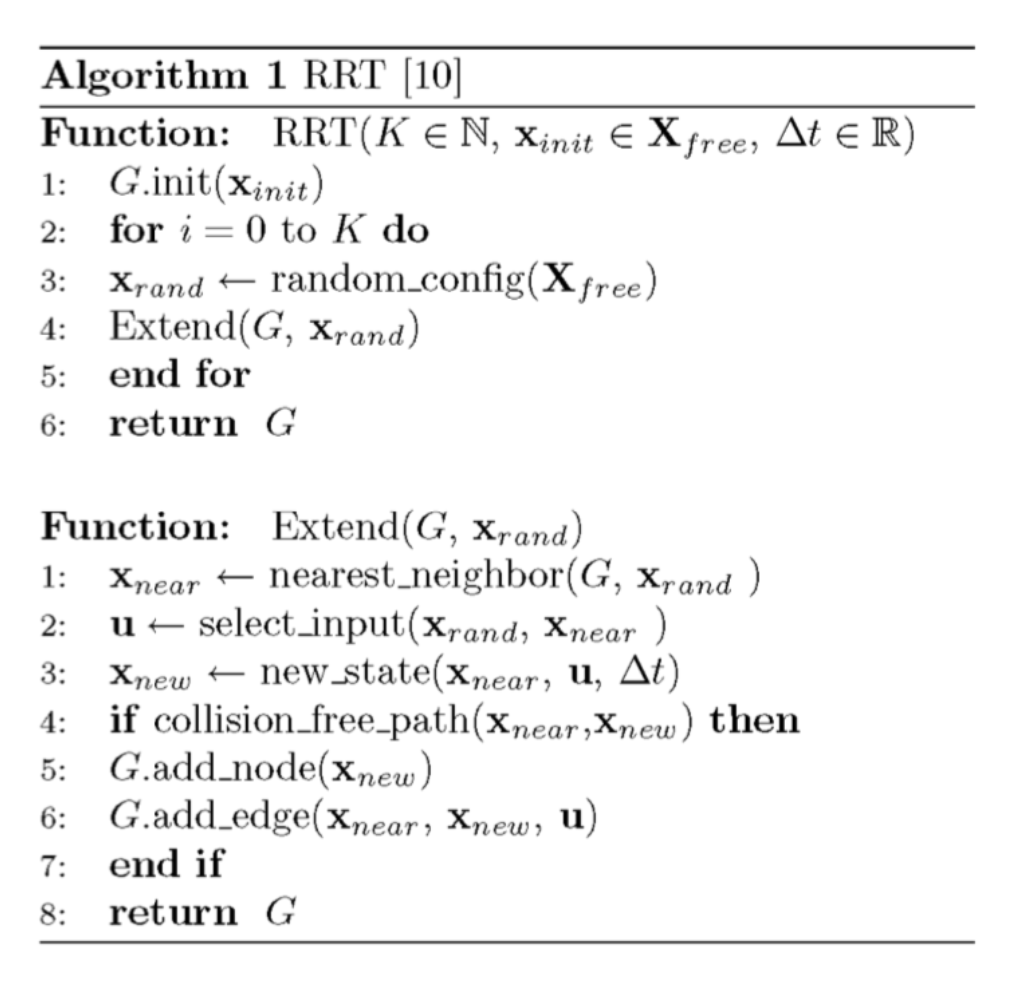
\includegraphics[scale=.4, angle =0]{figures/rrt_code.png}
    \caption{RRT Pseudo-code.}
    \label{RRT pseudocode}
\end{figure}

\begin{figure}[H]
    \centering
        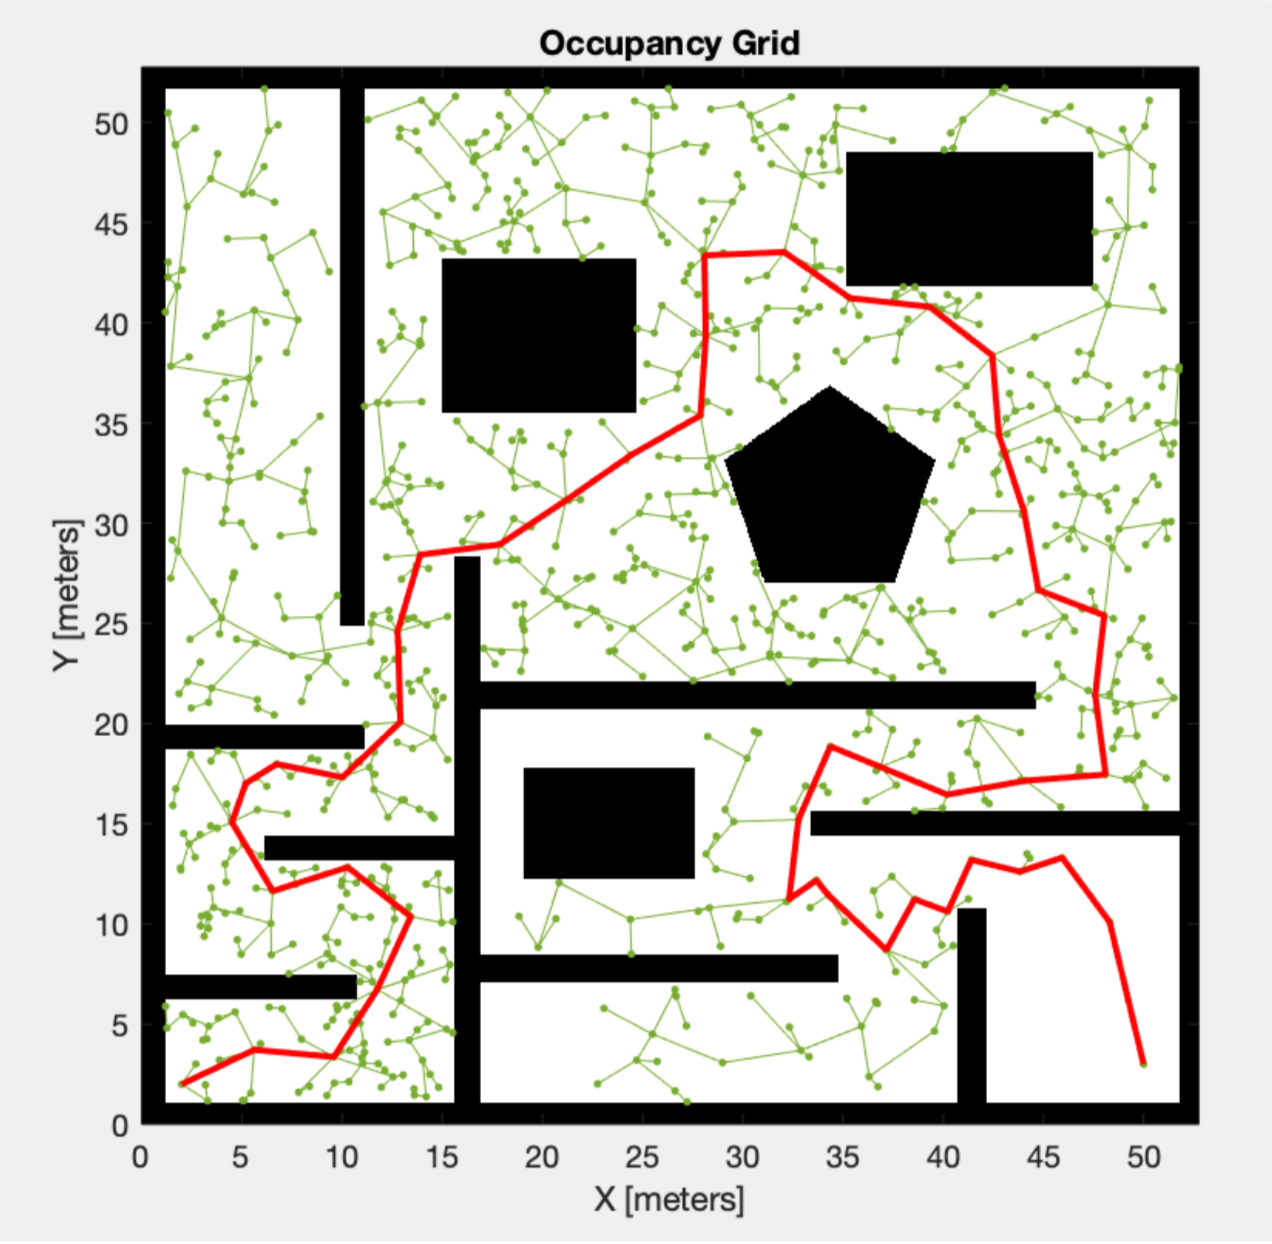
\includegraphics[scale=.3, angle =0]{figures/rrt-1.png}
    \caption{RRT Preliminary Testing Results.}
    \label{RRT Prelininary Results.}
\end{figure}

After preliminary testing of the RRT algorithm in an arbitrary map using Matlab, a potential problem surfaced that the path is always a zig-zagging pattern with sharp turning angles. Which means the robot needs to drive in a straight line, stop and turn in place before continuing onto the next section of the path. Though this motion is within the capability of the selected drive train, this kind of path is highly inefficient for indoor navigation, especially if the robot is in tracking motion with a certain desired camera facing angle. Therefore, a different implementation was made with the non-holonomic ackerman steering constraint for a more coherent path for the robot to follow. 
The non-holonomic RRT is similar to the state lattice planning where a minimum turning radius needs to be satisfied when connecting the existing frontier node to a potential new node. The figure below demonstrates the non-holonomic planning between nodes and the dynamic equations for calculating the robot arc trajectory given a steering angle.

\begin{figure}[H]
    \centering
        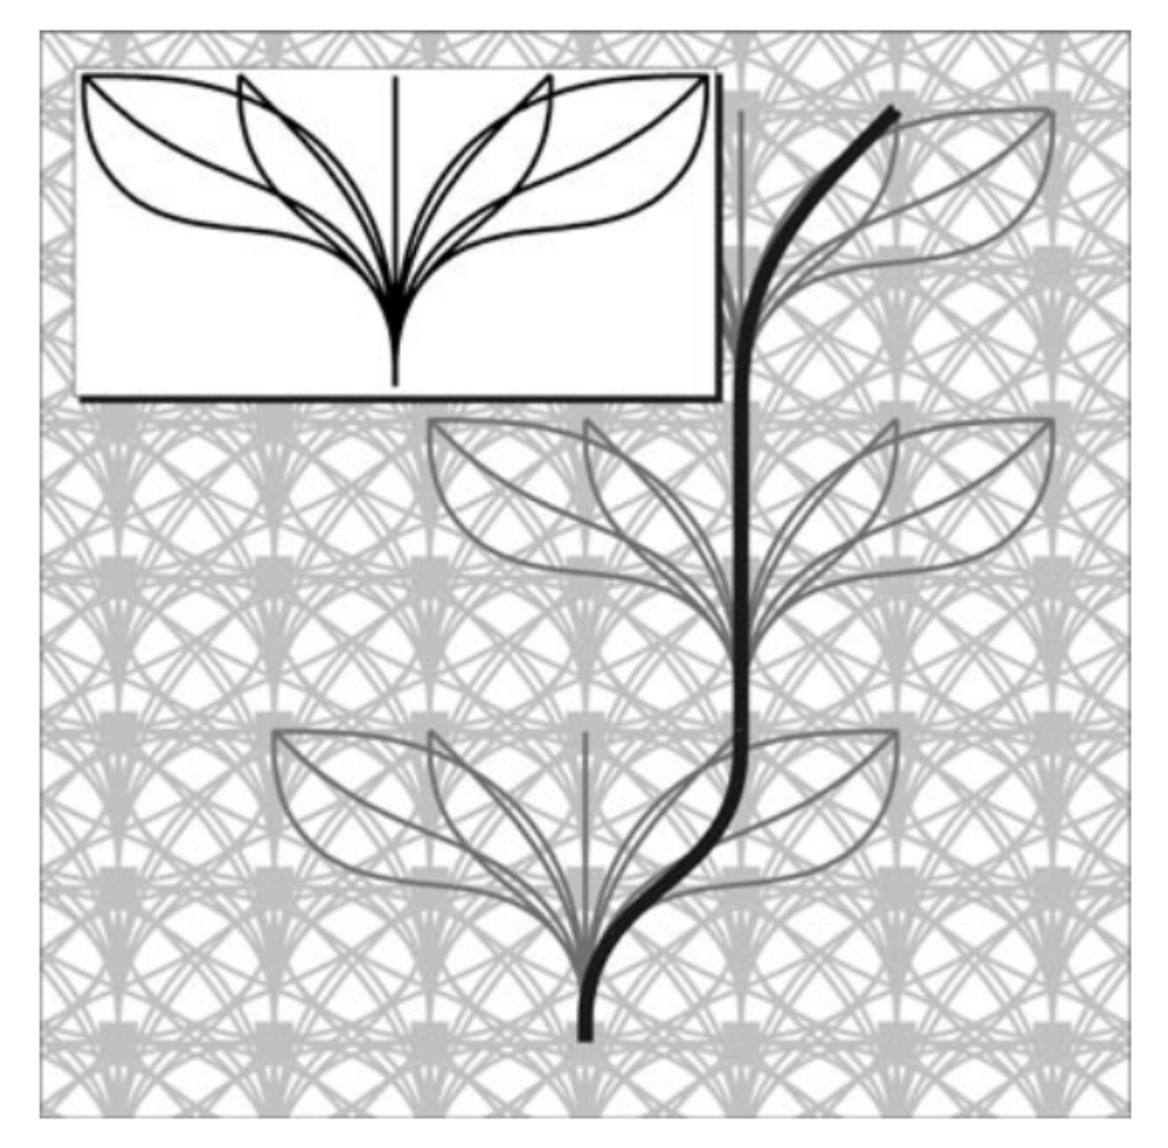
\includegraphics[scale=.3, angle =0]{figures/rrt-2.png}
    \caption{Non-holonomic Planning Between Nodes.}
    \label{Non-holonomic Planning Between Nodes.}
\end{figure}

\begin{figure}[H]
    \centering
        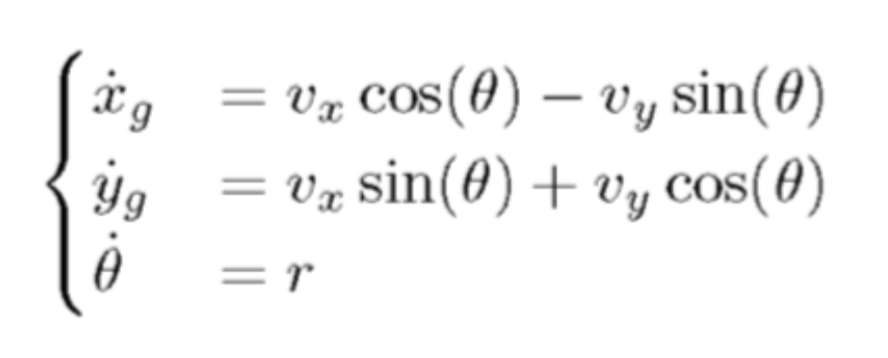
\includegraphics[scale=.4, angle =0]{figures/rrt-3.png}
    \caption{Non-holonomic Dynamic Equations.}
    \label{Non-holonomic Dynamic Equations.}
\end{figure}

\begin{figure}[H]
    \centering
        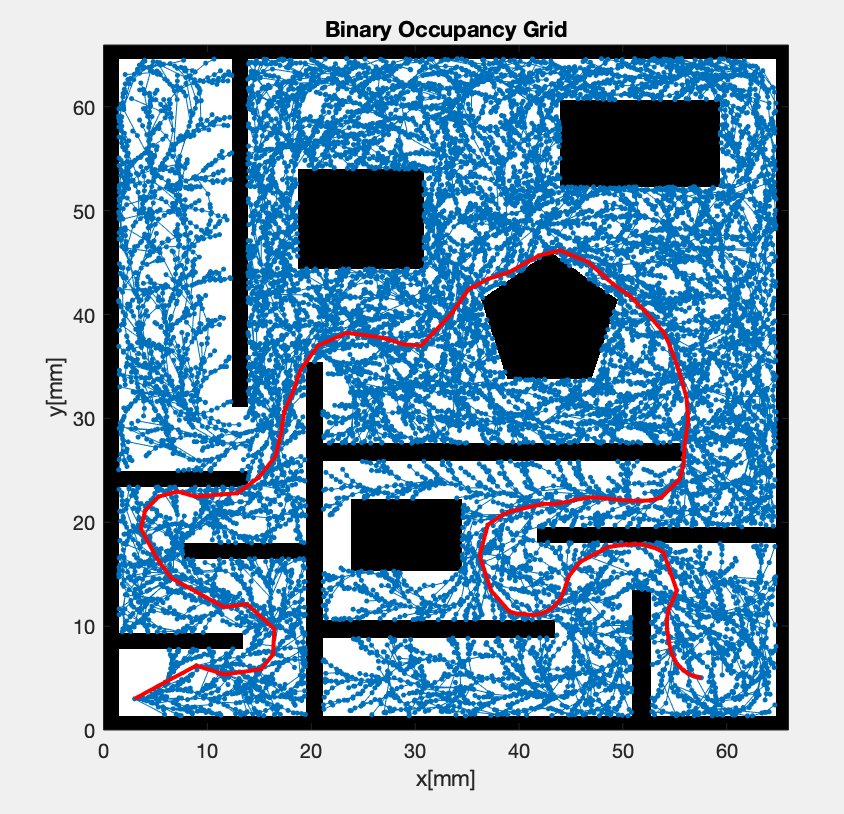
\includegraphics[scale=.5, angle =0]{figures/rrt-4.png}
    \caption{Non-holonomic RRT Preliminary Testing Results.}
    \label{Non-holonomic RRT Preliminary Testing Results}
\end{figure}

As it shows in the figure above, the resulting path is much more suitable for the robot to follow, however, with some sacrifice of the computing efficiency. More testing and optimization was conducted in larger indoor floor plan environments as shown in the figure below. The final path planning package takes in the current occupancy map of the environment, the odometry data from the localization and the end goal, then generates the path and sends via ROS as an array of waypoints. 

\begin{figure}[H]
    \centering
        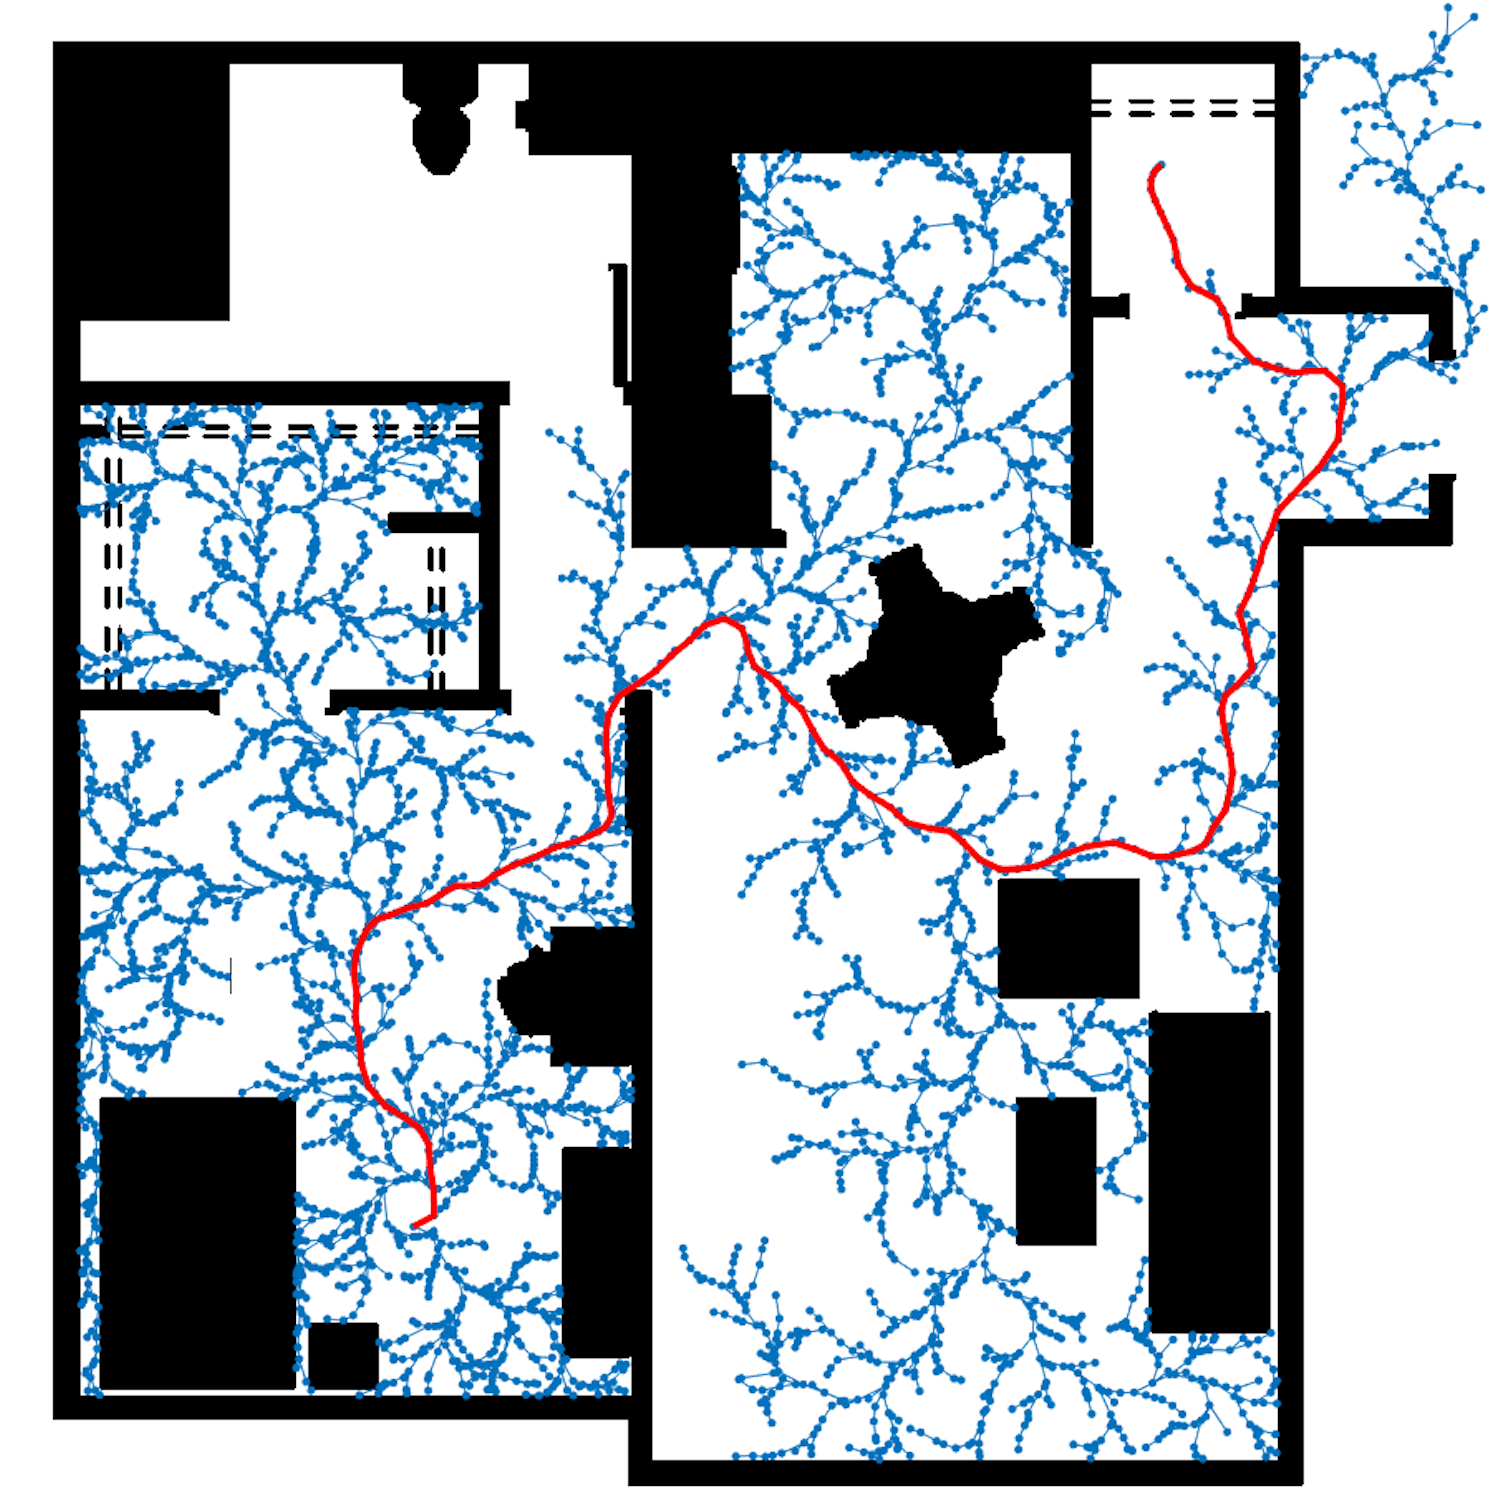
\includegraphics[scale=.3, angle =0]{figures/rrt-5.png}
    \caption{Non\-holonomic RRT Testing In Indoor Environment.}
    \label{Non-holonomic RRT Testing In Indoor Environment}
\end{figure}

For the local motion planning and the motion controller, a differential drive controller is implemented to provide velocity commands to the robot given arc radius and distance. However, due to time constraint, the team eventually chose to use the ROS navigation stack Action Lib as the motion controller as it also incorporated a local planner feature to deal with trajectory deviation and sudden obstacles using potential field local costmaps. 

\subsection{Launcher Trajectory Planning}
The trajectory planner module is the controlling where the robot navigates and when to launch a ball from . Figure \ref{Trajectory Planner High Level Flow} shows the trajectory planner operating in two modes: Navigation and Trajectory. During Navigation mode, the trajectory planner is passively generating launch waypoints and waiting for the system to navigate to the waypoint. 

During Trajectory mode, the navigation systems are passive and the trajectory planner attempts to compute safe trajectories to launch from. Additionally, the module consists of 2 subsystems: Trajectory Generator and Physics Model. The former subsystem allows for the creation and destruction of trajectories on the while operating. A flow control diagram of this system can be seen in Figure \ref{Trajectory Planner Generator Flow} below. The latter subsystem is a library that contains a Newtonian physics model that neglects air resistance. Air resistance was ignored due to the intended use of the tennis balls being launched. The key design parameters behind this decision are the: maximum speed of 6.7056 m/s, muzzle force of 3.33 N, and mass of the tennis ball being 49.8g; air resistance the projectile is negligible at this scale. 

During robot operations, the entertainer relies on a number of entertainer subsystems such as point cloud mapping, motion planner, and cameras. The flow of the Trajectory planner is shown in Figure \ref{Trajectory Planner High Level Flow}. The EnterTrainer will boot into navigation mode and begin to check on map availability from the navigation module. If the map is available, the trajectory planner will randomly select an X-Y coordinated way-point to launch from. The system will reference the map of its environment to check for collisions and ensure the path can be navigated too. If the system is unable to generate navigable points within a set time frame, the system defaults to a home position. During navigation, the trajectory planner module waits for the system to arrive at its destination before proceeding.

Once the Navigation mode has finished its routing, the system will transition to the Trajectory mode. In this mode, the system launcher starts generating trajectories as shown in figure Figure \ref{Trajectory Planner Generator Flow}. The system will record its current orientation X-Y plane and the the linear distance in the X-Z plane front on the robot. If the distance returned from the sensor is greater than the max distance the distance is set the max distance capable of being launched to. The system will then run the Trajectory Generator Subsystem which creates a list of trajectories generators functions and sends them to the point cloud subsystem to check for known collision points to avoid hitting objects. The priority of trajectories that are selected is determined by the maximum time of flight per trajectory. The collision check is performed by radius searching each trajectory point against the ball trajectory X-Z plane point cloud data using a Point Cloud Library (PCL) kd-tree. If no collision in a safe radius has been calculated, the trajectory parameters will be returned to the main operations loop. If a collision has been found, the impact energy that is imparted onto the hit object will be estimated. If the resulting impact energy is less than a predefined threshold, the trajectory will be marked as valid and returned to the system. If the previous conditions cannot be met, the trajectory is discarded and a new trajectory is selected from the available pool of trajectories. Finally, if the system runs out of generated trajectories, it will return failure causing the trajectory planner increment orientation in the X-Y plane in steps of 30 degrees. If the robot a turned 360 degrees, the system has no area where is can safely launch a ball and the system will revert to Navigation mode. However, if the safe trajectory has been calculated and confirmed, a signal is sent to the launcher system with relevant parameters to begin firing sequence.

\begin{figure}[H]
    \centering
        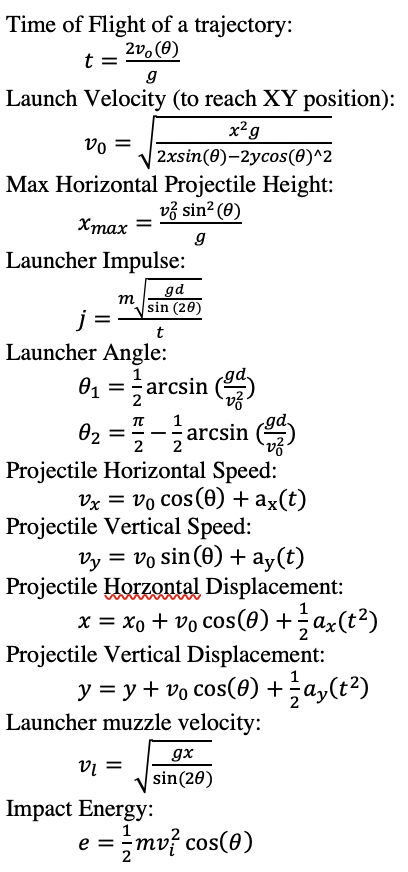
\includegraphics[scale=.40, angle =0]{figures/physics model.png}
    \caption{Newtonian physics equations used to calculate projectile flight of a tennis ball.}
    \label{Projectile Physics models}
\end{figure}

\begin{figure}[H]
    \centering
        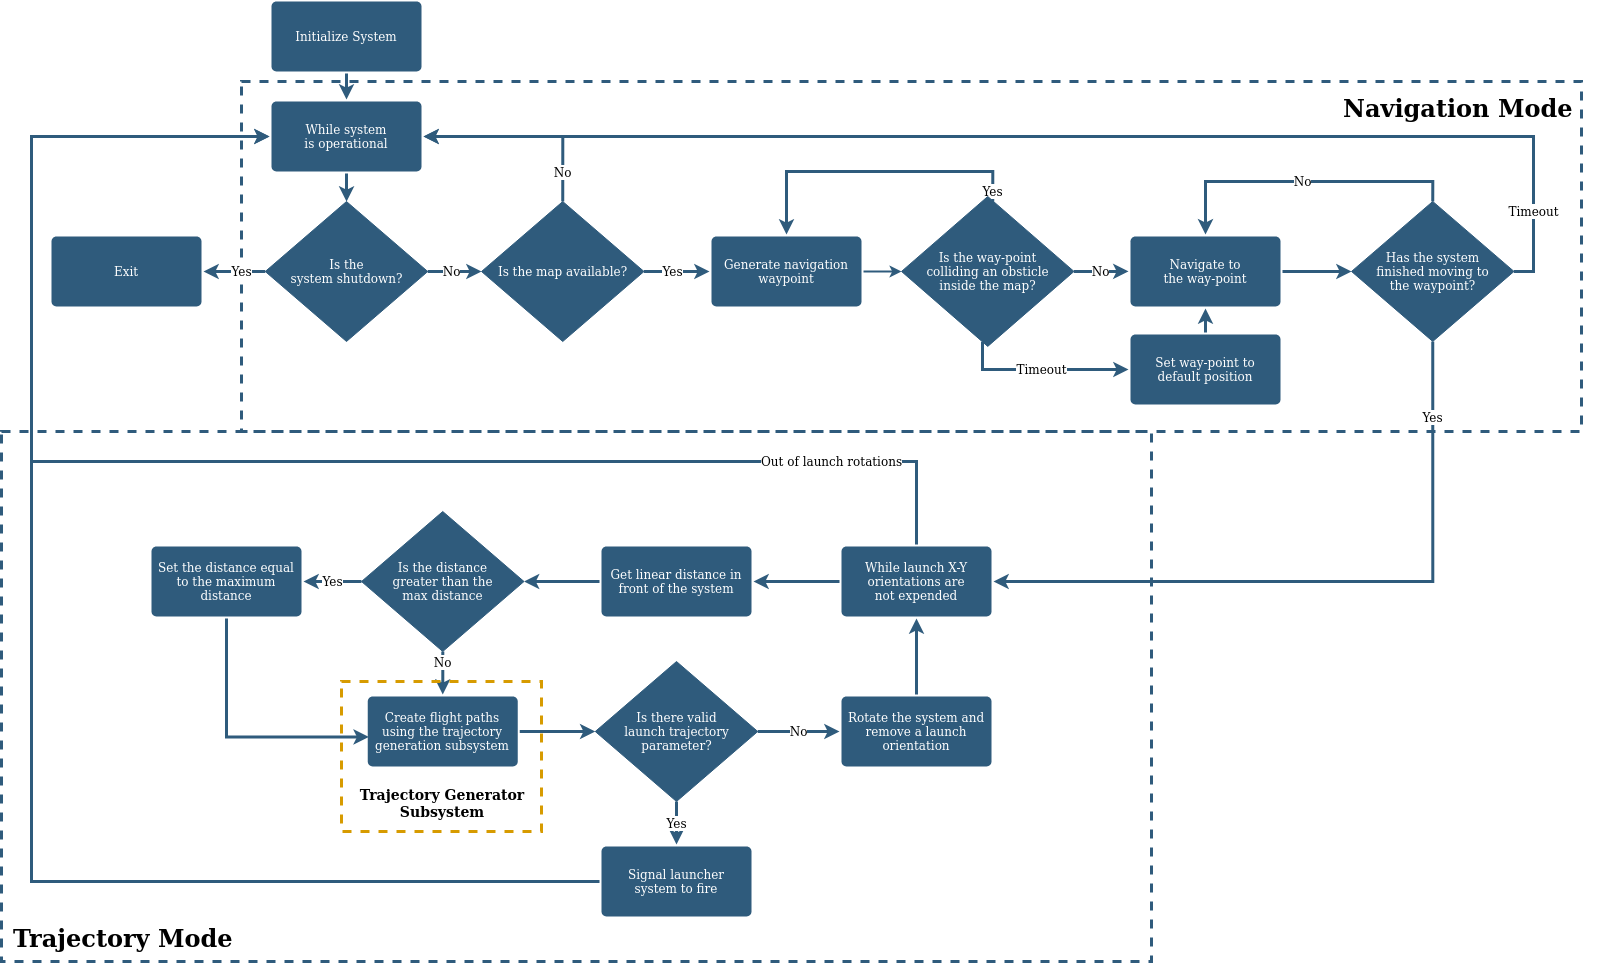
\includegraphics[scale=.35, angle =90]{figures/Trajectory Planner Diagrams.png}
    \caption{Flow control of the trajectory planner within the entertainer system.}
    \label{Trajectory Planner High Level Flow}
\end{figure}

\begin{figure}[H]
    \centering
        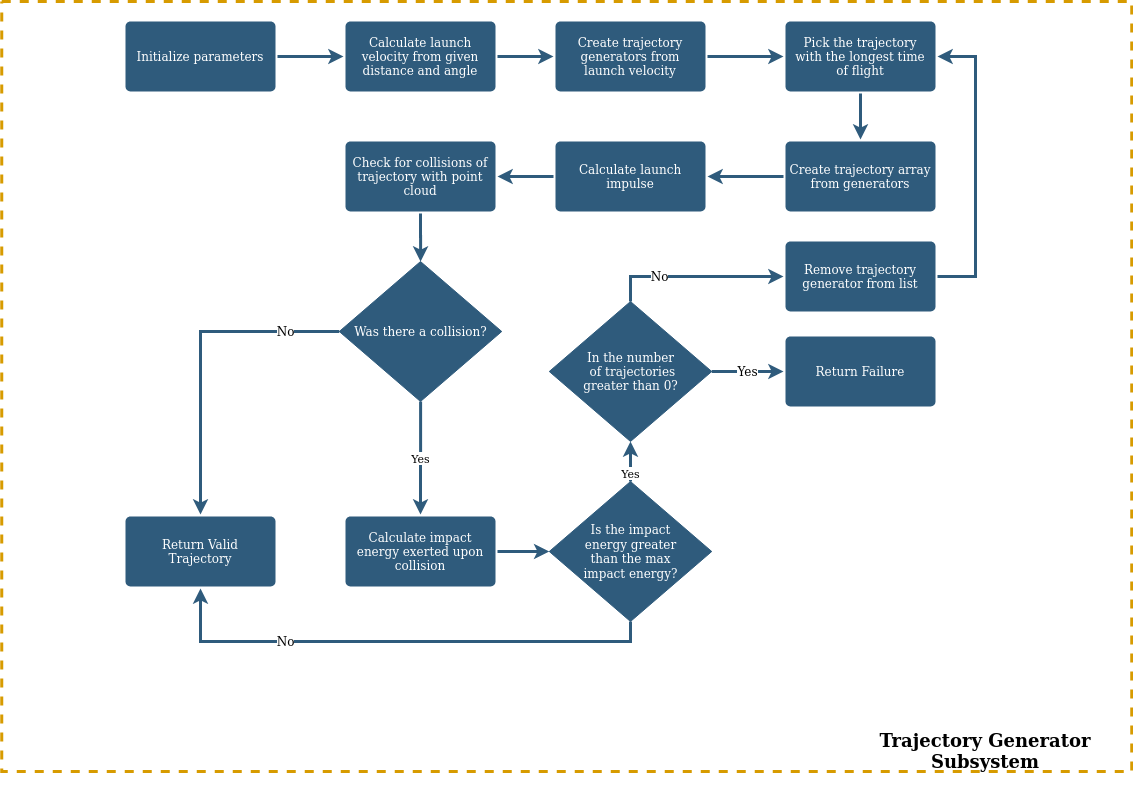
\includegraphics[scale=.35, angle =0]{figures/Trajectory Generatory Flow.png}
    \caption{Trajectory generator subsystem flow control.}
    \label{Trajectory Planner Generator Flow}
\end{figure}

% --------------------
\subsection{Launcher Controller}
For the purpose of this project the launcher controller was simulated.  In a real system the launcher controller would interface with a set of mechanical components to command the compression of the spring and the release of the electromagnet.  In order to accomplish the facility the launching sequence, a projectile be simulated in the environment with the launcher. The toy tennis ball that was selected is roughly 49.8 grams with a approximate radius of 0.01905 meters as seen in \ref{Dog Toy}.
%-- Add a photo of the "tennis ball"
\begin{figure}[H]
    \centering
        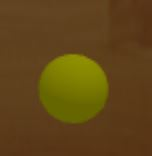
\includegraphics[scale=.4, angle =0]{figures/ball.JPG}
    \caption{Gazebo Representation of a Dog Toy Tennis Ball.}
    \label{Dog Toy}
\end{figure}
In the physical implementation the balls would be stored within a physical cavity or groove, but in the, simulation balls were stored above the launcher. The advantages of storing the balls in this manner eliminated the complexity of simulating the full set of physical characteristics of the robot system. It provided a means of visually verifying how many projectiles were in the queue to launch. It also reduced the number of required collision calculations by only having one projectile "loaded" into the launcher at a time.  The nature of the simulation is to provide a semi-realistic interaction of objects so the projectiles would interfere with each other if they touched.  
%-- Add a photo of the ball storage
\begin{figure}[H]
    \centering
        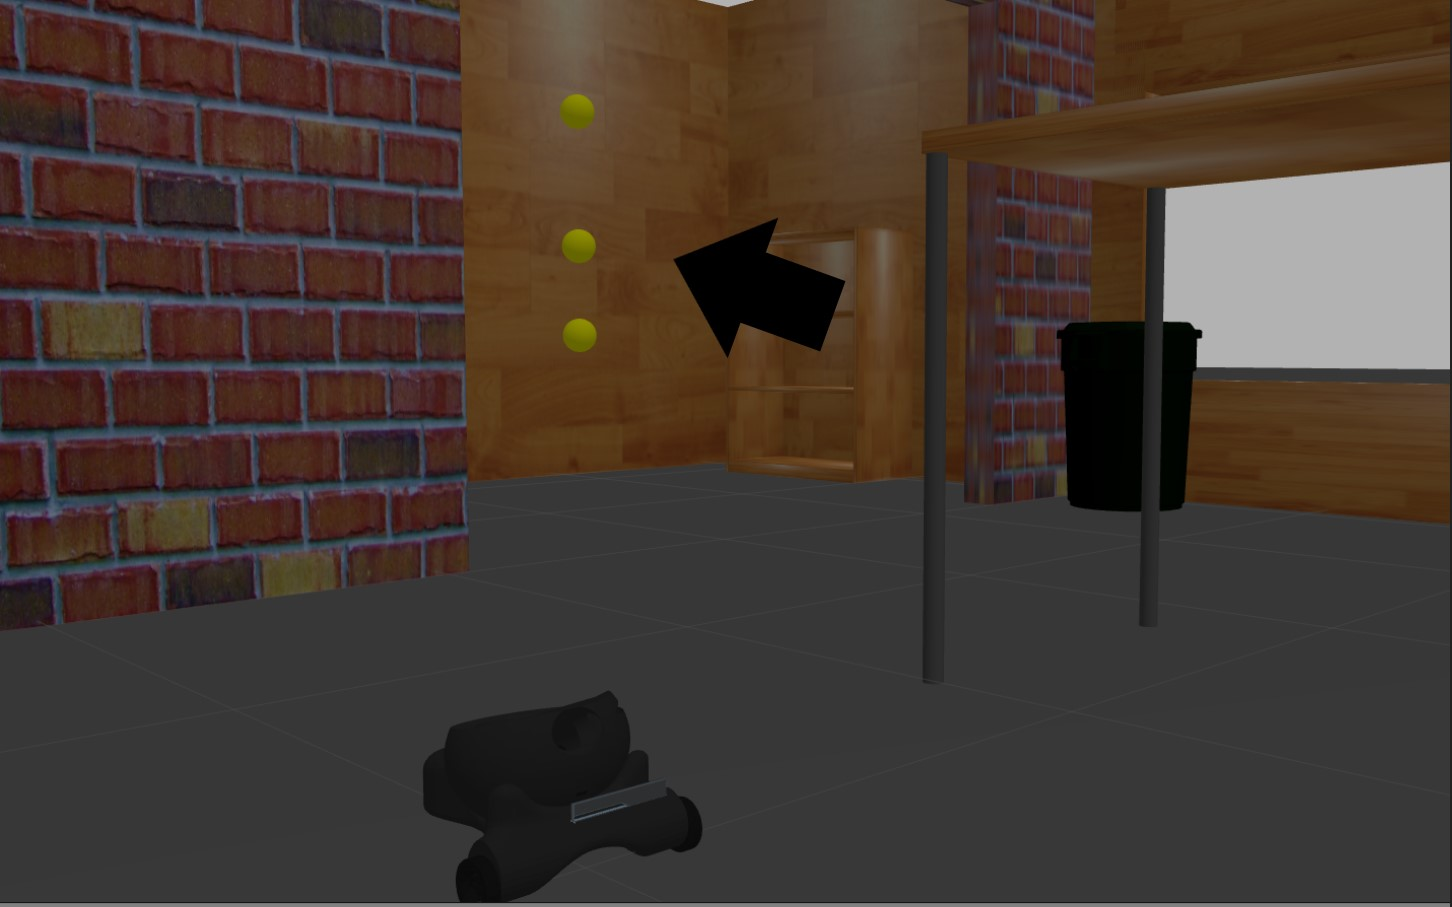
\includegraphics[scale=.2, angle =0]{figures/ball_storage.JPG}
    \caption{In order to simplify the physics of ball storage, the balls were stored above the robot.}
    \label{Simulated Ball Storage}
\end{figure}
The trajectory planner module provides not only an angle but also an impulse force calculation that can be applied to an object in the simulation.  In this case the impulse force is applied to a toy tennis ball which is described above.  To allow the Trajectory Planner to know when a ball was launched, the launcher angle, and how many balls are left a ROS message was used to package up that data and ship it back.  


% --------------------
\section{Simulation}
% --------------------
Many pieces of the EnterTrainer are able to be simulated in Gazebo and ROS.  Starting with a well tested framework like the Turtlebot (specifically the Turtlebot3 Waffle) the EnterTrainer was quickly stood up.  The trajectory calculation was verified with a measurement of the forward movement calculation of the ball compared to that of the simulated launched ball given an impulse force on the provided angle.  

One of the hurdles the team worked through was reference frames, since we were using an existing platform the reference frames were not developed cleanly from the start.  Specifically the point cloud data from the forward facing camera had a rotation that caused all following queries of the data to need a rotation.  To resolve this issue a new reference frame was created and the point cloud data was remapped to that new frame. This allowed easy query of data as well as easy visualization in RVIZ to verify the data.  Check out Figure \ref{Point Cloud Data and Trajectory in RVIZ} for representation of this data.  

\begin{figure}[H]
    \centering
        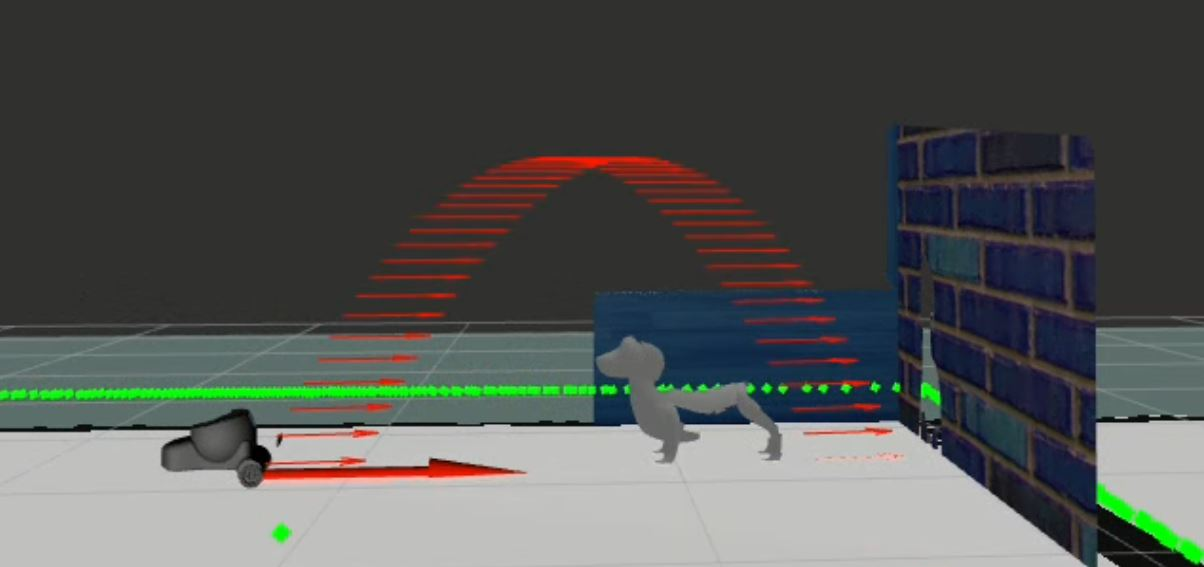
\includegraphics[scale=.4, angle =0]{figures/arc.JPG}
    \caption{The point cloud data provided to RVIZ along with an example trajectory for launching the tennis ball over a dog.  The blue brick wall on the right is actually from the depth data of the forward facing sensor.  The grey object in the middle is a representative dog model.  The Red arc is the plotted ball trajectory.  The Green dots forming approximate lines is from the 2D LiDAR data. }
    \label{Point Cloud Data and Trajectory in RVIZ}
\end{figure}

Through visual verification the EnterTrainer will dial back the force of the launch when facing close to a wall and if no safe trajectory is found it rotates like the algorithm was designed to do.  
The EnterTrainer navigates (Figure \ref{Navigation}) without wall collision to the selected point and orients itself in the requested orientation based off of the local cost map (Figure \ref{Cost Map}) and estimated system position/orientation.  

\begin{figure}[H]
    \centering
        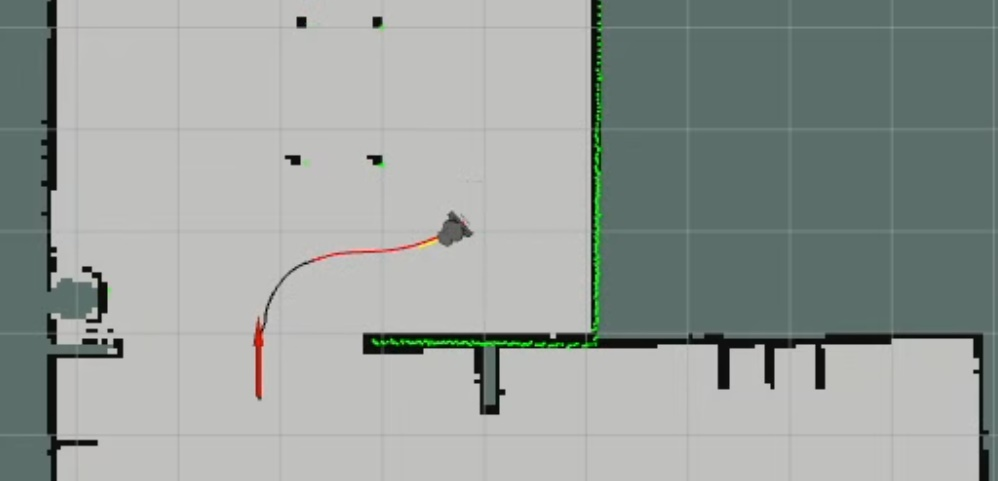
\includegraphics[scale=.4, angle =0]{figures/navigation.JPG}
    \caption{The robot navigation is visualized within the house map.  }
    \label{Navigation}
\end{figure}

\begin{figure}[H]
    \centering
        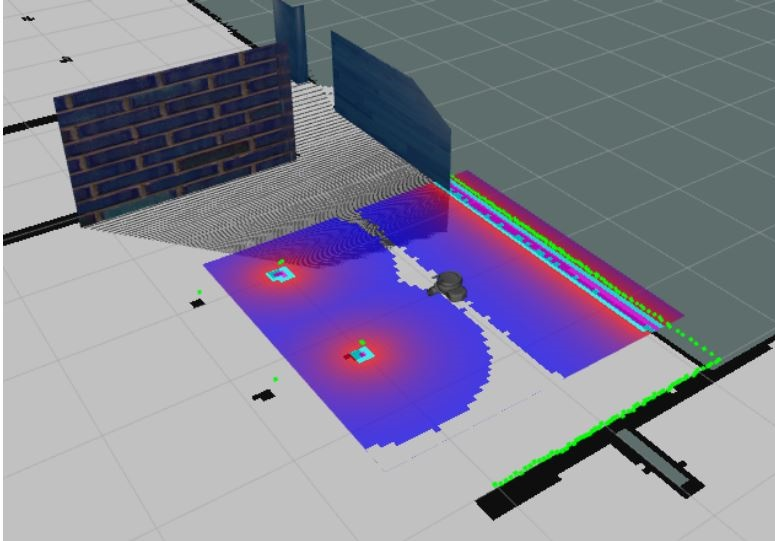
\includegraphics[scale=.4, angle =0]{figures/costmap.JPG}
    \caption{The local cost map based off of sensor data. }
    \label{Cost Map}
\end{figure}


% --------------------
\section{Discussion and Conclusions}
% --------------------

The EnterTrainer systems have many improvements that can be made. A few high level improvements are improved launcher range, decrease the energy sinks in the launcher (to increase system accuracy), trajectory planner object detection, and reduce computational complexity.  Through the time of this course the team grew to appreciate the process of systems engineering and the impact that has on other disciplines.  The team learned that it is important to have more upfront software design and architecture which resolves problems with integration and test.  For example, the team experienced issues with interfacing each module due to inconsistent definitions and structure of custom messages.  Moving forward the team would suggest stepping back and doing a top down analysis of architecture and interfaces to verify a clean and modular framework.  The team also sees the need for more prototyping and testing to verify and validate the trade studies. In conclusion the team met the objectives set forth above, the system was designed and simulated, and verification was conducted within the scope of the course.  


/

% %%%%%%%%%%%%%%%%%%%%%%%%%%%%%%%%%%%%%%%%%%%%%%%%%%%%%%%%%%
% %%%%%%%%%%%%%%%%%%%%%%%%%%%%%%%%%%%%%%%%%%%%%%%%%%%%%%%%%%
% REFERENCES SECTION
% %%%%%%%%%%%%%%%%%%%%%%%%%%%%%%%%%%%%%%%%%%%%%%%%%%%%%%%%%%
% %%%%%%%%%%%%%%%%%%%%%%%%%%%%%%%%%%%%%%%%%%%%%%%%%%%%%%%%%%
%References
%\bibliographystyle{IEEEtran}

\begin{thebibliography}{1}
\bibitem{c1}
Vidas et al. “3D Thermal Mapping of Building Interiors using an RGB-D and Thermal Camera”  Conference Paper in Proceedings - IEEE International Conference on Robotics and Automation · May 2013

\bibitem{c2}
Hornung, A., Wurm, K.M., Bennewitz, M. et al. OctoMap: an efficient probabilistic 3D mapping framework based on octrees. Auton Robot 34, 2013. 

\bibitem{c3}
Yguel, Manuel Aycard, Olivier Laugier, Christian. (2007). Update Policy of Dense Maps: Efficient Algorithms and Sparse Representation. Springer Tracts in Advanced Robotics. 

\bibitem{c4}
Gere, James M., and Barry J. Goodno. Mechanics of Materials. Cengage Learning, 2013.

\bibitem{c5}
Knight, Randall Dewey. Physics for Scientists and Engineers: a Strategic Approach. Pearson, Addison Wesley, 2008. 

\end{thebibliography}


\end{document}